\chapter{相关工作}

本章中主要介绍与本文相关的国内外工作,主要包括对变更影响域分析的子过程和相关工具的调研。
\section{程序间差异性分析}
\label{relate_diff}

对于软件演进分析而言,如何确定一个程序的不同版本之间的变更是一个关键性的问题\cite{kim2013identifying}。程序间差异性分析能够通过分析同一程序的不同版本间的差异,来确定版本间的变更集合\cite{lahiri2010differential,winstead2003towards}。

按分析的深度而言,程序间差异性分析可以分为三类:
\begin{itemize}
	\item 文本差异:单纯对比文本间的不同,这是最简单也最广泛应用的分析方法,如Unix Diff工具。
	\item 语法差异:对比并获得源代码间语法结构上的不同。
	\item 语义差异:对比并获得源代码间语义层面上的不同。
\end{itemize}

现有的帮助工程师进行软件维护和演进过程的工具往往都受限于低质量的变更信息。例如,源代码的变更信息往往都存储于版本管理系统中(如CVS)等,它们会追踪对某个特定文件的文本行的增加/删除等操作,但没有考虑代码中的结构化变更。

考虑到源代码能够以抽象语法树(Abstract Syntax Tree)的形式进行表达,可以采用树间差异分析的方法来抽取出这些变更信息。Change Distilling就是这样一类进行树间差异分析的算法\cite{fluri2007change,gall2009change}。该算法能够从两棵AST之间寻找匹配节点,并找到一个能够令一棵树转化为另一棵树的最小变更集合,该变更集合即为所求的程序间差异。而且由于是从AST中抽取信息,该算法可以获取语法结构上的变更信息。

Change Distilling中采用二元字符串相似性来匹配源代码语句,并使用子树相似性来匹配源代码结构(如语句、循环等)。在寻找变更集合时,它采用基本的树变更操作来描述源代码的变更,包括更新、删除、增加等。在实际的使用过程中,该算法可能会受限于如何找到数量合适的移动操作。

\section{程序变更影响分析}
\label{relate_impact}
软件维护是软件开发周期中最为复杂、成本最高的劳动密集型活动。软件产品需要跟随用户需求的变更而进行适应和变化,而软件变更可以帮助软件实现这种维护过程。事实上,软件变更是软件维护过程中的基础组件,它可能来自于新的需求、缺陷修复、变更请求等,然而将变更应用于软件时,它们会不可避免的带来一些副作用,导致可能会与原软件的其他部分发生冲突。

而变更影响分析(Change Impact Analysis)正是这样一类用于确定变更对于软件其他部分影响的技术集合\cite{li2013survey},它在软件开发、维护和测试等过程中都起到重要的作用\cite{acharya2011practical}。一般而言,变更影响分析可以用于程序理解、变更影响预测、影响追踪、变更传播、测试用例的选取等过程。

变更影响分析方法可以分类如下:
\begin{itemize}
	\item 基于可追踪性的变更影响分析\cite{de2008traceability},它追踪两个不同抽象级别的软件元素之间的依赖性,其目的在于链接不同类型的软件工件(如需求、设计等)。

	\item 基于依赖的变更影响分析\cite{law2003incremental},它致力于衡量变更的潜在影响,并试图分析程序语法结构间的关系,即程序实体间的语义依赖。这类变更影响分析主要在源代码级别进行研究。
\end{itemize}

软件变更可能导致意料之外的副作用,而变更影响分析的目的就在于找到这些副作用(Side Effect或者Ripple Effect)\cite{bohner1996software},并防止之。
变更影响分析从分析变更请求和源代码开始,最后能够得到估计影响集合(Estimated Impact Set),与真实影响集合(Actual Impact Set)相比该结果可能存在一定的误差。

整个软件变更影响分析的过程可以大致划分为如下流程\cite{de2008traceability,bohner2002software},更详细的流程可以参考图\ref {变更影响分析process}。

%\begin{enumerate}
%	\item 
	该分析过程需要输入变更集合,然后对变更请求进行分析。该步骤即特征定位(feature location),用于找到源代码中相应功能的起始实现位置\cite{biggerstaff1993concept}。该分析过程将衡量变更集合引入的影响。该步骤是目前大部分变更影响分析技术的重点,其主要的两类包括:
%	\item 
	
	\begin{itemize}
	
	\item 静态分析:包括历史分析、文本分析、结构分析等\cite{sun2012comparative,kagdi2007survey}。静态分析主要分析程序的语法、语义或者历史依赖,容易产生许多误报(False Positive)。
		\begin{itemize}
		\item 结构分析着重于分析程序间的结构依赖性并构建依赖关系图
		\item 文本分析根据程序中的注释和标识符提取出其概念依赖性
		\item 历史分析能够从多个软件版本的演进过程中挖掘相关信息
		\end{itemize}
%		\begin{figure}[H]
%			\centering
%			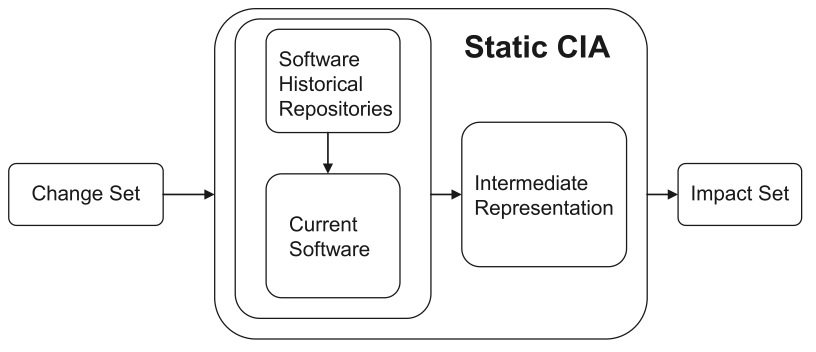
\includegraphics{chap02_02}
%			\caption {静态分析过程}
%		\end{figure}
	
	\item 动态分析:包括在线分析和离线分析。该分析过程需要给出特定输入,并依赖程序运行时所收集到的信息来进行分析(如运行时的路径追踪和覆盖信息等)\cite{law2003whole}。该分析过程所得到的影响集合往往比静态分析的精度更高,但其开销也相应更大,且容易错报(False Negative)。
%		\begin{itemize}
%		\item 在线变更影响分析使用程序运行时收集的信息来进行
%		\end{itemize}
		
%		\begin{figure}[H]
%			\centering
%			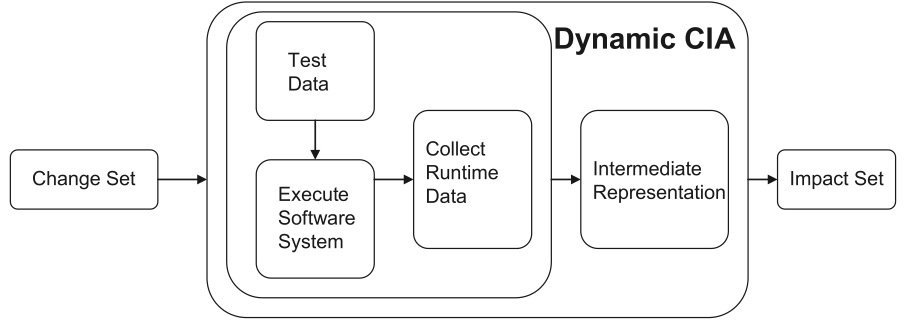
\includegraphics{chap02_03}
%			\caption {动态分析过程}
%		\end{figure}	

		
	\end{itemize}
%\end{enumerate}

\begin{figure}[H]
	\centering
	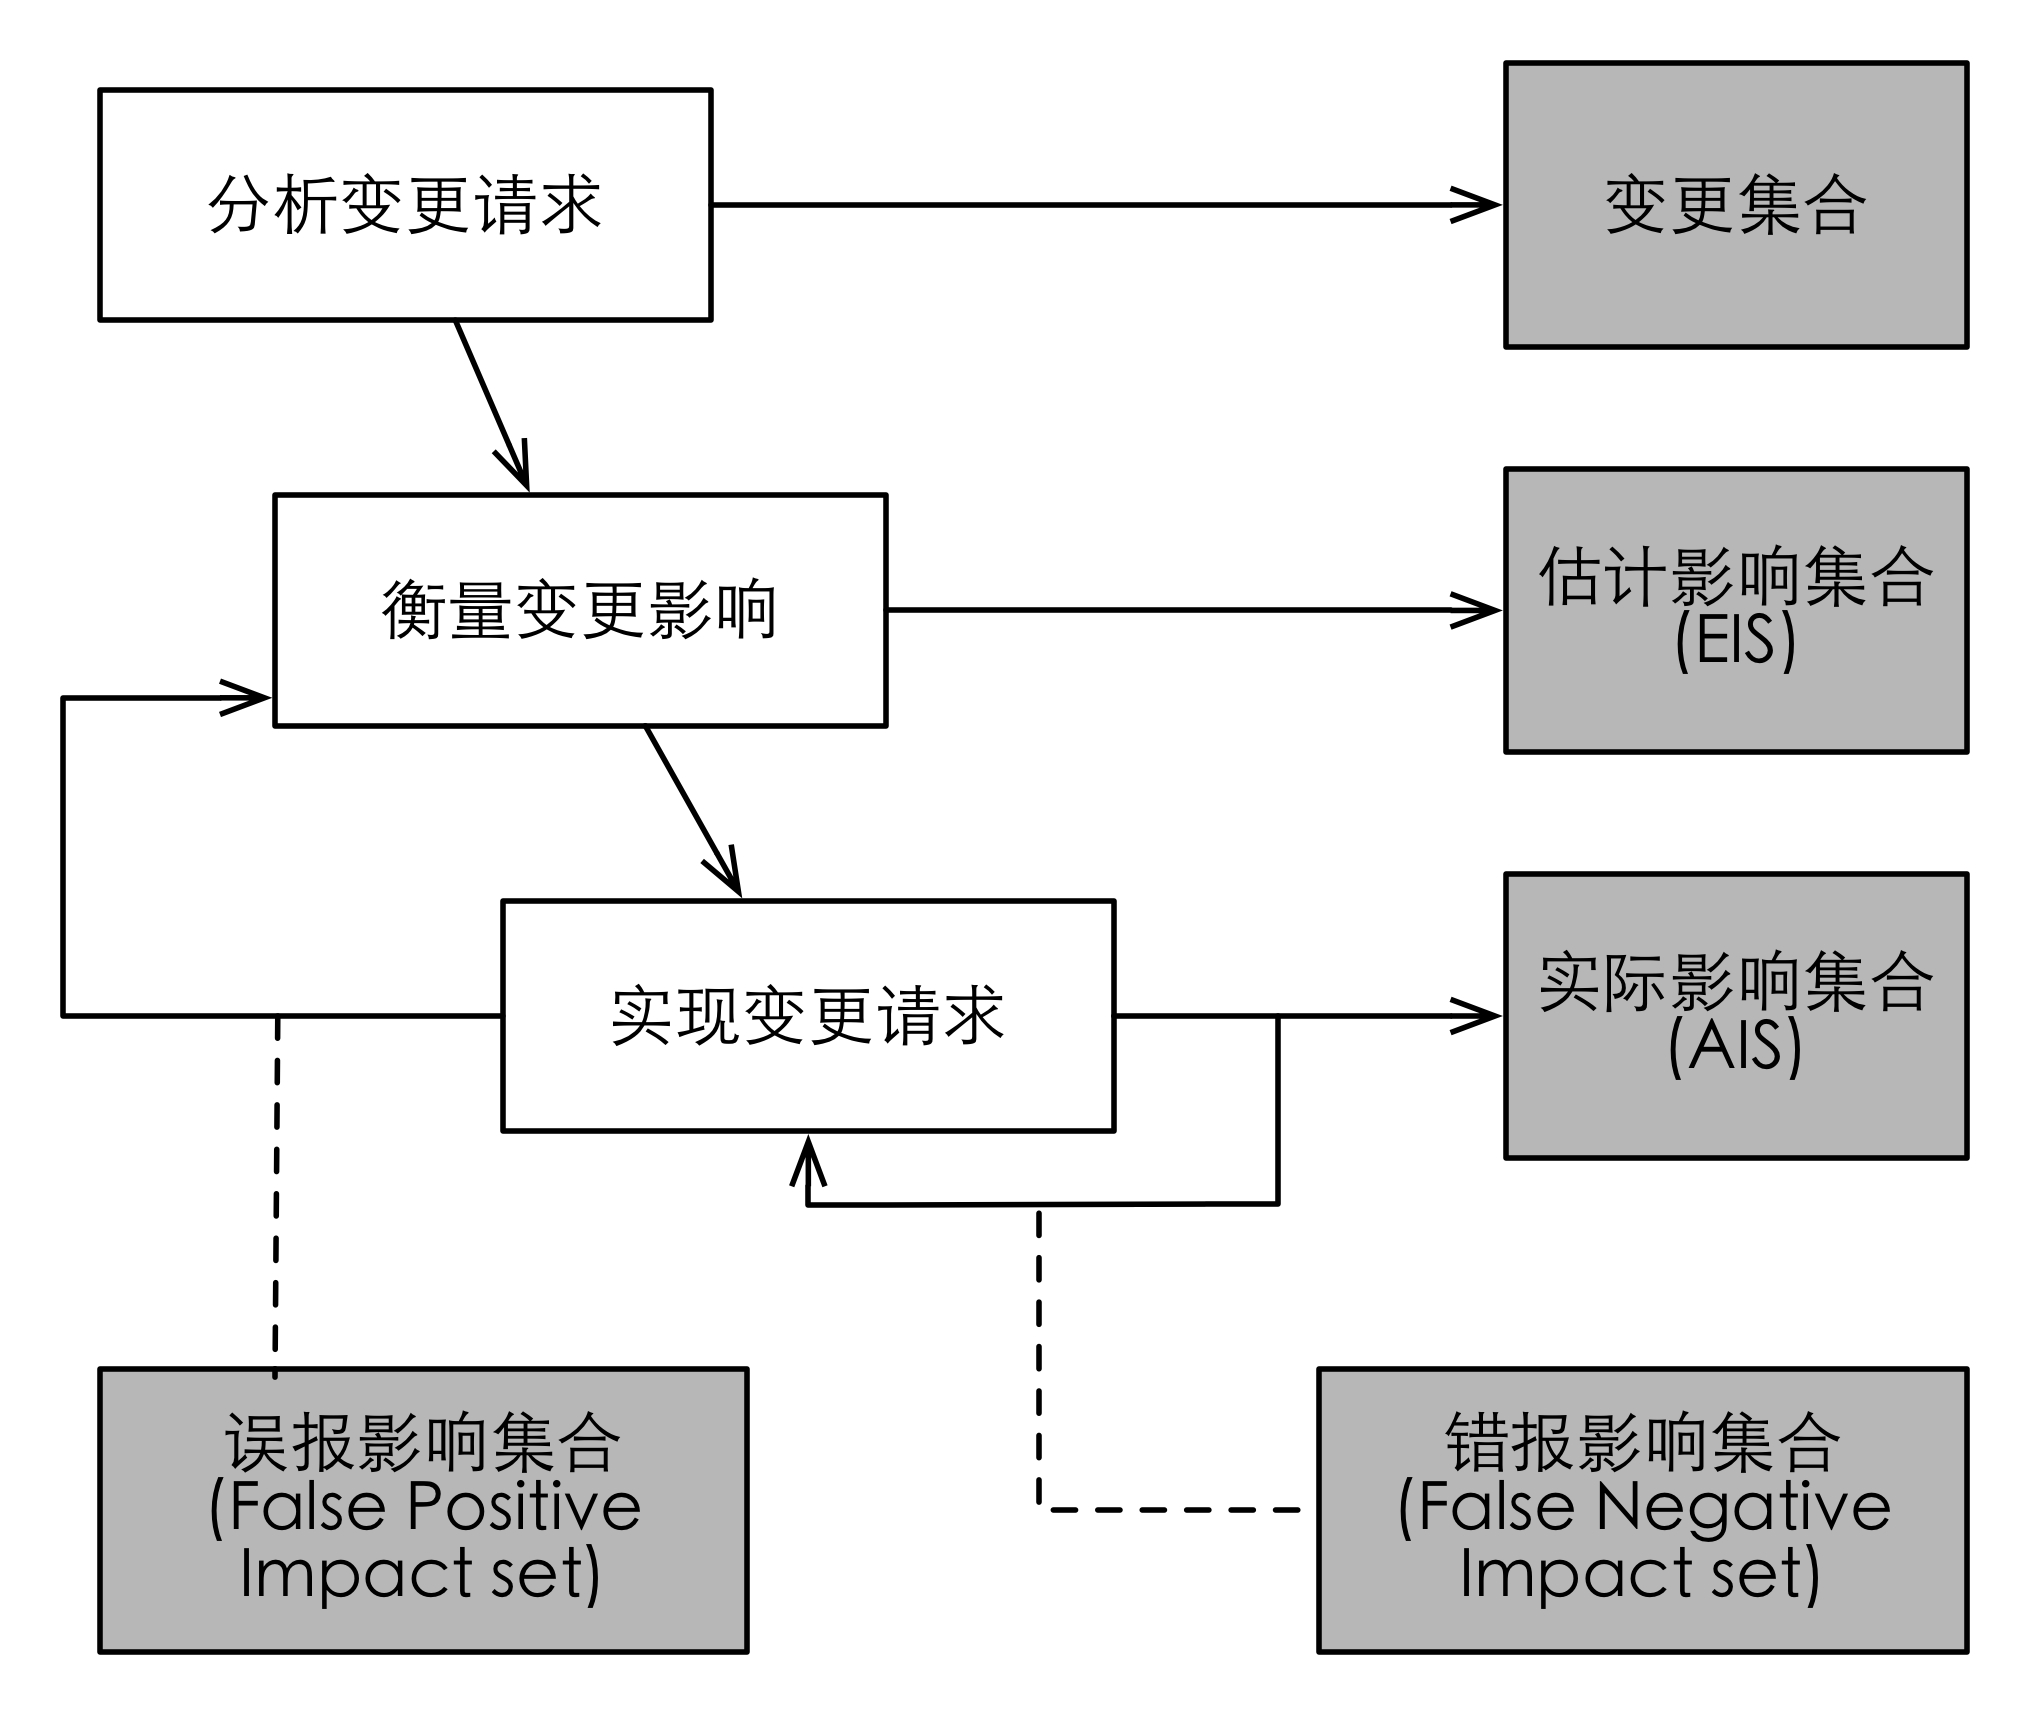
\includegraphics[height=.6\columnwidth]{chap02_01.jpg}
	\caption {变更影响分析过程}
	\label {变更影响分析process} 
\end{figure}

近年来,学术界中实现了某些以变更影响分析技术为支撑的工具,这些工具通常会利用变更影响分析得到的影响集合来完成后续的分析过程,帮助软件进行维护和演进。下面给出相关的简要介绍:
\begin{itemize}
	\item Chianti:支持Java语言,可作为Eclipse插件使用\cite{ren2004chianti}。该工具首先使用回归测试来分析变更前的程序是否能正常使用,若回归测试失败,则利用Chianti工具实施变更影响分析,该分析过程通过将软件变更拆分成若干原子变更来分析变更之间的依赖关系。最后结合原程序生成某种中间表示形式并找到可能影响到测试用例运行的代码位置。
	
	\item JRipples:支持Java语言,可作为Eclipse插件使用\cite{buckner2005jripples,rajlich2004incremental}。该工具利用依赖关系图自动标注可能被变更的类所影响的其他类,并提示用户其变更的可能影响传播路径。该工具的分析结果可进行人工修正。
	
	\item ROSE:支持用CVS工具进行版本管理的Java项目,可作为Eclipse插件使用\cite{zimmermann2005mining}。该工具需要挖掘软件代码仓库,当用户对代码进行变更时,提示用户某些其他变更可能与之相关(其形式类似于“变更了该函数的人通常还变更了另一个函数”)。
	
	\item jpf-regression:支持Java语言,可用作Eclipse插件或直接作为命令行工具使用\cite{person2011directed}。该工具利用程序切片技术进行变更影响分析,使用得到的影响集合来驱动符号化执行,找到可能被变更影响到的程序行为。
\end{itemize}



\section{相关工具}
\label{relate_tool}
	本节主要介绍实验采用的相关工具。
	

	\subsection{git}		

git是一个分布式的版本控制系统,最初由 Linus Torvalds在2005年为Linux内核而开发,现在已经成为最流行的版本控制系统。

与CVS和SVN等集中式的C/S版本控制系统不同,git是一种分布式的版本管理系统,每个本地git工作目录都具有完整的历史数据和版本追踪能力,无需网络连接或服务器端的支持。
      
本文主要采用git作为版本管理与合并的工具。

	\subsection{Beyond Compare}
		
Beyond Compare 是一款内容比较工具,可用于文件、目录、压缩包等数据间的比较,横跨Windows、Mac OS X和Linux三大操作系统,可用作常见版本控制系统的第三方文本比较与合并工具。
      
本文主要采用该工具作为文本比较和合并工具,用于解决补丁版本迁移时可能遇到的冲突。


	\subsection{jpf-regression} 
变更影响分析常用于衡量软件变更的潜在影响,其分析结果通常可用做其他程序分析技术的输入,例如回归测试可利用变更影响分析来确定程序的哪些部分需要进行再分析。由于单行变更就足以引发广泛的未知影响,变更影响分析在软件的演进和维护过程中扮演着重要的角色。\cite{rungta2012change}

目前,大部分的自动分析工具都以程序语法结构的形式描述变更的影响,如函数和语句等。基于依赖的分析方法一般通过分析程序组件间的内部关系来衡量变更的影响,这类技术通常使用程序位置信息来描述变更的影响,缺失了受影响代码位置的相关运行路径信息。这类信息往往对程序行为的验证、调试等工作帮助很大,而且能够将需要关注的代码范围缩小,使得只需关注受影响的程序行为集合即可。

(Directed Incremental Symbolic Execution )DiSE\cite{person2011directed,yang2014directed}方法能够结合静态分析的效率和符号化执行的精度等优点,该方法能分析限制在方法内部的变更影响,并描述程序变更对其行为的影响。

jpf-regression是DiSE方法的工具实现,它基于Java Path Finder框架\cite{havelund2000model}实现,支持Java语言,可作为Eclipse的插件使用。本文将采用该工具来实现变更语义影响分析过程。下面对该方法中的影响分析算法进行简介。

DiSE方法采用程序切片技术来衡量变更对代码中其他部分的影响,其生成的影响集合可以用于引导符号化执行来分析受变更影响的程序行为,并生成相应的路径条件(Path Condition),这些路径条件描述了受影响的程序行为,在分析结束后可以利用SMT等技术进行路径求解,用于后续的验证、调试等过程。

在DiSE方法中,程序变更影响分析是其后续分析过程的基础,其变更影响分析技术的主要特点包括:
\begin{enumerate}
	\item 粒度:基本块。即变更影响分析过程中,以基本块为单位进行影响集合的计算。
	\item 影响范围:方法内部。即将单次影响集合计算的范围局限于方法内部,最后得到变更对其所属方法内部的其他语句所造成的影响。
	\item 影响来源:主要从控制流和数据流两个方面考虑变更所造成的影响,采用语句间的控制依赖和数据依赖关系进行影响计算。
\end{enumerate}

DiSE方法中的影响集合主要分为两类:
\begin{itemize}
	\item ACN:受影响的条件语句节点(Affected Conditional Nodes)。
	\item AWN:受影响的赋值语句节点(Affected Write Nodes)。
\end{itemize}

为了得到这两类影响集合,DiSE中使用四条规则进行迭代计算。从原始的变更集合出发,不断应用规则向外扩展,最后得到的闭包即为所求的影响集合:
\begin{enumerate}
	\item 如果ACN中有一个节点$n_i$,且存在一个条件节点$n_j$,其中$n_j$控制依赖于$n_i$,那么将$n_j$加入到ACN中。
	\item 如果nj是一条赋值语句,且控制依赖于ACN中的节点$n_i$,那么$n_j$加入到AWN中。
	     
%	前两条公式表明,如果条件语句和赋值语句控制依赖于变更后的CFG中的节点,那么他们就应当被加进来。
%	     
	\item 如果AWN中的一条赋值语句节点$n_i$对于变量的赋值在条件语句$n_j$中被使用了,且CFG中存在一条从$n_i$到$n_j$的路径,那么将$n_j$加入到ACN中。

	\item 如果一个写语句节点$n_i$对于对于变量的赋值在AWN或ACN中的某个节点$n_j$被使用了,且CFG中存在一条从$n_i$到$n_j$的路径,那么将$n_i$加入到AWN中。

\end{enumerate}



\subsection{ASTro}	

	本文采用的程序间语法差异性分析工具是由内布拉斯加大学林肯分校的Josh Reed,Suzette Person和Sebastian Elbaum等人所开发的ASTro,它是jpf-regression工具自带的前置工具,用于比对两个不同版本的源代码并获取其抽象语法树上的差异,并将得到的变更集合以XML格式输出。该工具支持Java语言。
	
\section{本章小结}
本章主要介绍了相关的国内外工作。
章节\ref{relate_diff}介绍了程序间差异性分析的相关工作。
章节\ref{relate_impact}介绍了变更影响分析的相关工作。
章节\ref{relate_tool}介绍了本文中所用到的相关工具。
	